\documentclass[tikz,border=6pt]{standalone}
\usepackage[T1]{fontenc}
\usepackage[utf8]{inputenc}
\usepackage{tikz}
\usetikzlibrary{
  arrows.meta,
  calc,
  positioning,
  shapes.geometric,
  shapes.misc
}
\usepackage{xcolor}

\definecolor{regiongreen}{HTML}{DCEFD9}
\definecolor{regiongray}{HTML}{ECECEC}
\definecolor{regionyellow}{HTML}{F7EFCB}

\tikzset{
  >=Latex,
  line/.style={draw=black, thick, -Latex},
  conn/.style={draw=black, thick},
  block/.style={
    draw=black,
    fill=white,
    rectangle,
    rounded corners=1.5pt,
    align=center,
    inner sep=5pt
  },
  stage/.style={block, minimum width=26mm, minimum height=22mm},
  longstage/.style={block, minimum width=38mm, minimum height=22mm},
  keyblock/.style={block, minimum width=32mm, minimum height=18mm},
  sum/.style={draw=black, fill=white, circle, inner sep=0pt, minimum size=10mm, line width=1pt},
  explabel/.style={font=\small\bfseries, align=center},
  sublabel/.style={font=\small, align=center},
  tinylabel/.style={font=\footnotesize, align=center}
}


\begin{document}
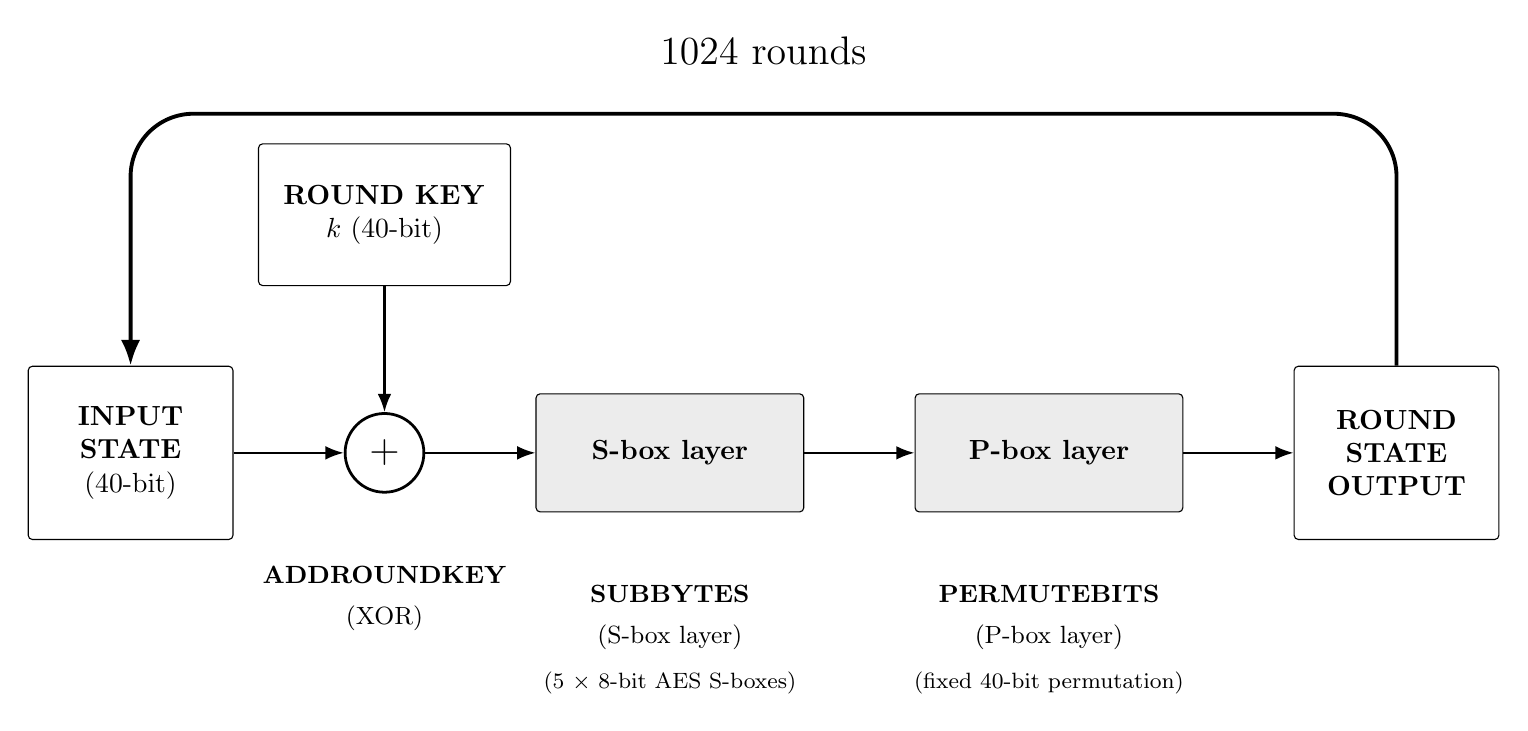
\begin{tikzpicture}[node distance=10mm and 12mm]
  \node[stage] (input) {\textbf{INPUT}\\\textbf{STATE}\\(40-bit)};
  \node[sum, right=14mm of input] (xor) {\Large $+$};
  \node[keyblock, above=16mm of xor] (key) {\textbf{ROUND KEY}\\$k$ (40-bit)};

  \node[block, fill=regiongray, minimum width=34mm, minimum height=15mm, right=14mm of xor] (subbox) {\textbf{S-box layer}};

  \node[block, fill=regiongray, minimum width=34mm, minimum height=15mm, right=14mm of subbox] (perm) {\textbf{P-box layer}};

  \node[stage, right=14mm of perm] (output) {\textbf{ROUND}\\\textbf{STATE}\\\textbf{OUTPUT}};

  \draw[line] (input) -- (xor);
  \draw[line] (key.south) -- (xor.north);
  \draw[line] (xor) -- (subbox);
  \draw[line] (subbox) -- (perm);
  \draw[line] (perm) -- (output);

  \coordinate (loopRightStem) at ($(output.north)+(0,24mm)$);
  \coordinate (loopRightTop) at ($(output.north)+(-8mm,32mm)$);
  \coordinate (loopLeftTop) at ($(input.north)+(8mm,32mm)$);
  \coordinate (loopLeftStem) at ($(input.north)+(0,24mm)$);
  \draw[line, line width=1.4pt]
    (output.north) -- (loopRightStem)
    (loopRightStem) to[out=90,in=0] (loopRightTop)
    (loopRightTop) -- (loopLeftTop)
    (loopLeftTop) to[out=180,in=90] (loopLeftStem)
    (loopLeftStem) -- (input.north);
  \node[font=\Large] at ($(loopLeftTop)!0.5!(loopRightTop)+(0,8mm)$) {1024 rounds};

  \node[explabel, below=8mm of xor] {ADDROUNDKEY};
  \node[sublabel, below=13mm of xor] {(XOR)};

  \node[explabel, below=8mm of subbox] {SUBBYTES};
  \node[sublabel, below=13mm of subbox] {(S-box layer)};
  \node[tinylabel, below=19mm of subbox] {(5 $\times$ 8-bit AES S-boxes)};

  \node[explabel, below=8mm of perm] {PERMUTEBITS};
  \node[sublabel, below=13mm of perm] {(P-box layer)};
  \node[tinylabel, below=19mm of perm] {(fixed 40-bit permutation)};
\end{tikzpicture}
\end{document}
